\section{Introduction}
This work is submitted in partial fulfilment of the course CS120: Computer network at ShanghaiTech University. The network stack is an essential topic in computer networks and has various implementations. To comprehensively understand it, we are asked to implement our network stack Athernet. \par
Unlike traditional wireless or wired methods, Athernet uses sound waves to transmit data between devices. The stack has implemented the basic functionalities of the standard TCP/IP and can be used with existing network infrastructure. Additionally, the system has the potential to be used in areas where wireless communication is not feasible, such as underwater communications.\par
\begin{figure}[H]
  \begin{center}
    \centerline{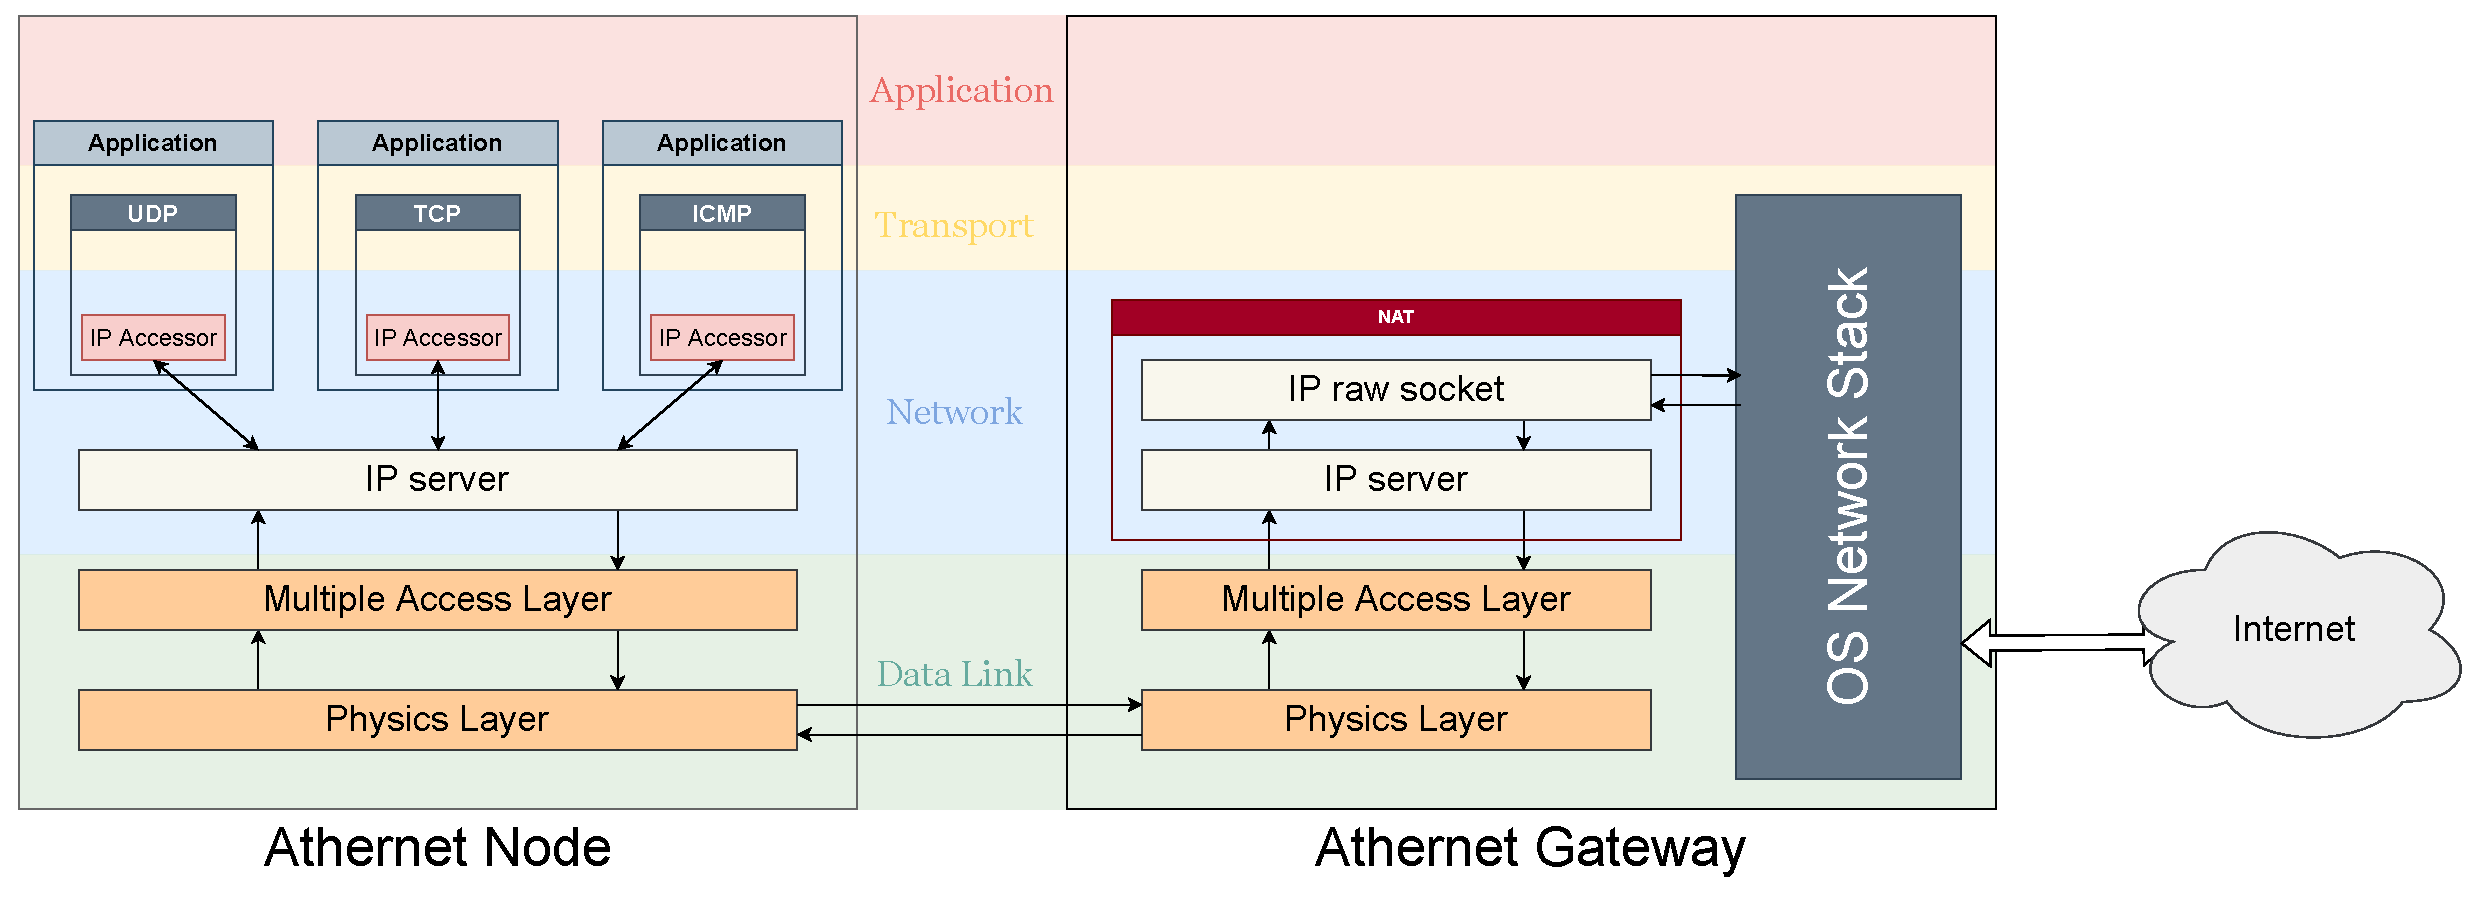
\includegraphics[width=\columnwidth]{./figures/overview.pdf}}
    \caption{the overview architecture of the Athernet network stack}
    \label{overview}
  \end{center}
\end{figure}

The network stack is composed of four layers, as follows:
\begin{itemize}
  \item \textbf{The link layer:} The link layer includes mainly two subparts:  \emph{physicas layer} and \emph{multiple access layer}. The physical layer is responsible for modulating the data and transferring the data through audio waves. It supports both transmitting through the air and the audio cable. Two different modulation schemes are implemented for the two scenarios: passband transmission using a combination of \emph{BPSK} and \emph{OFDM}, and baseband transmission using \emph{4B5B} with \emph{NRZI}. The multiple access layer deals with the collision. It uses \emph{CSMA/CA} to ensure that multiple peers can transfer data reliably.
  \item \textbf{The network layer:} In the internet layer, we implement the  \emph{Internet Protocol(IP)}. IP packets are received and sent to other layers through \emph{IP server} and \emph{IP accessor}. The \emph{network address translation(NAT)} are defined over IP server.
  \item \textbf{The transport layer:}The transport layer is composed of \emph {internet control message protocol(ICMP)}, \emph{user datagram protocol(UDP)} and \emph{transmission control protocol(TCP)}. We implement the full functionality for UDP and basic functionality for TCP.
  \item \textbf{The application layer:} We implemented \emph{file transfer protocol(FTP)} and built a simple acoustic FTP client. The proxy tunnelling is also implemented to support other network applications running on Athernet.
\end{itemize}
Figure~\ref{overview} shows the overall architecture of the Athernet. The Athernet nodes are interconnected and can connect to the Internet through the Athernet gateway, which runs a NAT.\par
% We select Rust as our main programing language due to its reliability and efficiency.
The paper is devided into five parts. Through chapter two to five, we describes the design of the four layers of our network stack. In the last chapter, we analyze the problems in our design and make a technical summary.